% Copyright 2008 by Till Tantau
%
% This file may be distributed and/or modified
%
% 1. under the LaTeX Project Public License and/or
% 2. under the GNU Free Documentation License.
%
% See the file doc/generic/pgf/licenses/LICENSE for more details.


\section{Chains}
\label{section-chains}

\begin{tikzlibrary}{chains}
    This library defines options for creating chains.
\end{tikzlibrary}
%
\begin{codeexample}[setup code,hidden]
    \usetikzlibrary{chains}
\end{codeexample}


\subsection{Overview}

\emph{Chains} are sequences of nodes that are -- typically -- arranged in a row
or a column and that are -- typically -- connected by edges. More generally,
they can be used to position nodes of a branching network in a systematic
manner. For the positioning of nodes in rows and columns you can also use
matrices, see Section~\ref{section-matrices}, but chains can also be used to
describe the connections between nodes that have already been connected using,
say, matrices. Thus, it often makes sense to use matrices for the positioning
of elements and chains to describe the connections.


\subsection{Starting and Continuing a Chain}

Typically, you construct one chain at a time, but it is permissible to
construct multiple chains simultaneously. In this case, the chains must be
named differently and you must specify for each node which chain it belongs to.

The first step toward creating a chain is to use the |start chain| option.

\begin{key}{/tikz/start chain=\opt{\meta{chain name}}\opt{\meta{direction}}}
    This key should, but need not, be given as an option to a scope enclosing
    all nodes of the chain. Typically, this will be a |scope| or the whole
    |tikzpicture|, but it might just be a path on which all nodes of the chain
    are found. If no \meta{chain name} is given, the default value |chain| will
    be used instead.

    The key starts a chain named \meta{chain name} and makes it \emph{active},
    which means that it is currently being constructed. The |start chain| can
    be issued only once to activate a chain, inside a scope in which a chain is
    active you cannot use this option once more (for the same chain name). The
    chain stops being active at the end of the scope in which the |start chain|
    command was given.

    Although chains are only locally active (that is, active inside the scope
    the |start chain| command was issued), the information concerning the
    chains is stored globally and it is possible to \emph{continue} a chain
    after a scope has ended. For this, the |continue chain| option can be used,
    which allows you to reactivate an existing chain in another scope.

    The \meta{direction} is used to determine the placement rule for nodes on
    the chain. If it is omitted, the current value of the following key is
    used:
    %
    \begin{key}{/tikz/chain default direction=\meta{direction} (initially going right)}
        This \meta{direction} is used in a |chain| option, if no other
        \meta{direction} is specified.
    \end{key}

    The \meta{direction} can have two different forms:
    \declare{|going |\meta{options}} or \declare{|placed |\meta{options}}. The
    effect of these rules will be explained in the description of the
    |on chain| option. Right now, just remember that the \meta{direction} you
    provide with the |chain| option applies to the whole chain.

    Other than this, this key has no further effect. In particular, to place
    nodes on the chain, you must use the |on chain| option, described next.
    %
\begin{codeexample}[]
\begin{tikzpicture}[start chain]
  % The chain is called just "chain"
  \node [on chain] {A};
  \node [on chain] {B};
  \node [on chain] {C};
\end{tikzpicture}
\end{codeexample}

\begin{codeexample}[]
\begin{tikzpicture}
  % Same as above, using the scope shorthand
  { [start chain]
    \node [on chain] {A};
    \node [on chain] {B};
    \node [on chain] {C};
  }
\end{tikzpicture}
\end{codeexample}

\begin{codeexample}[]
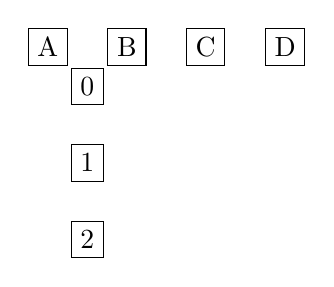
\begin{tikzpicture}[start chain=1 going right,
                    start chain=2 going below,
                    node distance=5mm,
                    every node/.style=draw]
  \node [on chain=1] {A};
  \node [on chain=1] {B};
  \node [on chain=1] {C};

  \node [on chain=2] at (0.5,-.5) {0};
  \node [on chain=2] {1};
  \node [on chain=2] {2};

  \node [on chain=1] {D};
\end{tikzpicture}
\end{codeexample}
    %
\end{key}

\begin{key}{/tikz/continue chain=\opt{\meta{chain name}}\opt{\meta{direction}}}
    This option allows you to (re)activate an existing chain and to possibly
    change the default direction. If the |chain name| is missing, the name of
    the innermost activated chain is used. If no chain is activated, |chain| is
    used.

    Let us have a look at the two different applications of this option. The
    first is to change the direction of a chain as it is being constructed. For
    this, just give this option somewhere inside the scope of the chain.
    %
\begin{codeexample}[]
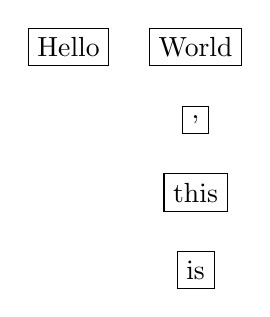
\begin{tikzpicture}[start chain=going right,node distance=5mm]
  \node [draw,on chain] {Hello};
  \node [draw,on chain] {World};
  \node [draw,continue chain=going below,on chain] {,};
  \node [draw,on chain] {this};
  \node [draw,on chain] {is};
\end{tikzpicture}
\end{codeexample}

    The second application is to reactivate a chain after it ``has already been
    closed down''.
    %
\begin{codeexample}[]
\begin{tikzpicture}[node distance=5mm,
                    every node/.style=draw]
  { [start chain=1]
    \node [on chain] {A};
    \node [on chain] {B};
    \node [on chain] {C};
  }

  { [start chain=2 going below]
    \node [on chain=2] at (0.5,-.5) {0};
    \node [on chain=2] {1};
    \node [on chain=2] {2};
  }

  { [continue chain=1]
    \node [on chain] {D};
  }
\end{tikzpicture}
\end{codeexample}
    %
\end{key}


\subsection{Nodes on a Chain}

\begin{key}{/tikz/on chain=\opt{\meta{chain name}}\opt{\meta{direction}}}
    This key should be given as an option to a node. When the option is used,
    the \meta{chain name} must be the name of a chain that has been started
    using the |start chain| option. If \meta{chain name} is the empty string,
    the current value of the innermost activated chain is used. If this option
    is used several times for a node, only the last invocation ``wins''. (To
    place a node on several chains, use the |\chainin| command repeatedly.)

    The \meta{direction} part is optional. If present, it sets the direction
    used for this node, otherwise the \meta{direction} that was given to the
    original |start chain| option is used (or of the last |continue chain|
    option, which allows you to change this default).

    The effects of this option are the following:
    %
    \begin{enumerate}
        \item An internal counter (there is one local counter for each chain)
            is increased. This counter reflects the current number of the node
            in the chain, where the first node is node 1, the second is node 2,
            and so on.

            The value of this internal counter is globally stored in the macro
            \declare{|\tikzchaincount|}.
        \item If the node does not yet have a name, (having been given using
            the |name| option or the name-syntax), the name of the node is set
            to \meta{chain name}|-|\meta{value of the internal chain counter}.
            For instance, if the chain is called |nums|, the first node would
            be named |nums-1|, the second |nums-2|, and so on. For the default
            chain name |chain|, the first node is named |chain-1|, the second
            |chain-2|, and so on.
        \item Independently of whether the name has been provided automatically
            or via the |name| option, the name of the node is globally stored
            in the macro \declare{|\tikzchaincurrent|}.
        \item Except for the first node, the macro
            \declare{|\tikzchainprevious|} is now globally set to the name of
            the node of the previous node on the chain. For the first node of
            the chain, this macro is globally set to the empty string.
        \item Except possibly for the first node of the chain, the placement
            rule is now executed. The placement rule is just a \tikzname\
            option that is applied automatically to each node on the chain.
            Depending on the form of the \meta{direction} parameter (either the
            locally given one or the one given to the |start chain| option),
            different things happen.

            First, it makes a difference whether the \meta{direction} starts
            with |going| or with |placed|. The difference is that in the first
            case, the placement rule is not applied to the first node of the
            chain, while in the second case the placement rule is applied also
            to this first node. The idea is that a |going|-direction indicates
            that we are ``going somewhere relative to the previous node''
            whereas a |placed| indicates that we are ``placing nodes according
            to their number''.

            Independently of which form is used, the \meta{text} inside
            \meta{direction} that follows |going| or |placed| (separated by a
            compulsory space) can have two different effects:
            %
            \begin{enumerate}
                \item If it contains an equal sign, then this \meta{text} is
                    used as the placement rule, that is, it is simply executed.
                \item If it does not contain an equal sign, then
                    \meta{text}|=of \tikzchainprevious| is used as the
                    placement rule.
            \end{enumerate}

            Note that in the first case, inside the \meta{text} you have access
            to |\tikzchainprevious| and |\tikzchaincount| for doing your
            positioning calculations.
            %
\begin{codeexample}[]
\begin{tikzpicture}[start chain=circle placed {at=(\tikzchaincount*30:1.5)}]
  \foreach \i in {1,...,10}
    \node [on chain] {\i};

  \draw (circle-1) -- (circle-10);
\end{tikzpicture}
\end{codeexample}
        \item The following style is executed:
            %
            \begin{stylekey}{/tikz/every on chain}
                This key is executed for every node on a chain, including the
                first one.
            \end{stylekey}
    \end{enumerate}

    Recall that the standard placement rule has a form like
    |right=of (\tikzchainprevious)|. This means that each new node is placed to
    the right of the previous one, spaced by the current value of
    |node distance|.
    %
\begin{codeexample}[]
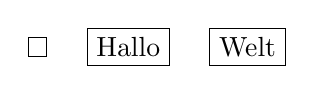
\begin{tikzpicture}[start chain,node distance=5mm]
  \node [draw,on chain] {};
  \node [draw,on chain] {Hallo};
  \node [draw,on chain] {Welt};
\end{tikzpicture}
\end{codeexample}

    The optional \meta{direction} allows us to temporarily change the direction
    in the middle of a chain:
    %
\begin{codeexample}[]
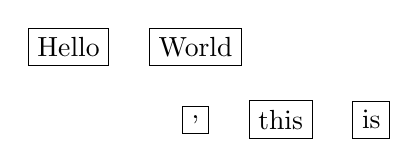
\begin{tikzpicture}[start chain,node distance=5mm]
  \node [draw,on chain] {Hello};
  \node [draw,on chain] {World};
  \node [draw,on chain=going below] {,};
  \node [draw,on chain] {this};
  \node [draw,on chain] {is};
\end{tikzpicture}
\end{codeexample}

    You can also use more complicated computations in the \meta{direction}:
    %
\begin{codeexample}[]
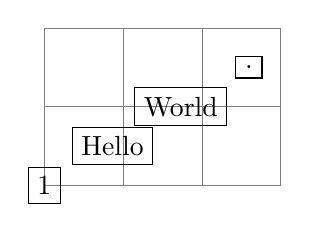
\begin{tikzpicture}[start chain=going {at=(\tikzchainprevious),shift=(30:1)}]
  \draw [help lines] (0,0) grid (3,2);
  \node [draw,on chain] {1};
  \node [draw,on chain] {Hello};
  \node [draw,on chain] {World};
  \node [draw,on chain] {.};
\end{tikzpicture}
\end{codeexample}
    %
\end{key}

For each chain, two special ``pseudo nodes'' are created.

\begin{predefinednode}{\meta{chain name}-begin}
    This node is the same as the first node on the chain. It is only defined
    after a first node has been defined.
\end{predefinednode}

\begin{predefinednode}{\meta{chain name}-end}
    This node is the same as the (currently) last node on the chain. As the
    chain is extended, this node changes.
\end{predefinednode}

The |on chain| option can also be used, in conjunction with |late options|, to
add an already existing node to a chain. The following command, which is only
defined inside scopes where a |start chain| option is present, simplifies this
process.

\begin{command}{\chainin |(|\meta{existing name}|)| \opt{\oarg{options}}}
    This command makes it easy to add a node to chain that has already been
    constructed. This node may even be part of a another chain.

    When you say |\chainin (some node);|, the node |some node| must already
    exist. It will then be made part of the current chain. This does not mean
    that the node can be changed (it is already constructed, after all), but
    the |join| option can be used to join |some node| to the previous last node
    on the chain and subsequent nodes will be placed relative to |some node|.

    It is permissible to give the |on chain| option inside the \meta{options}
    in order to specify on which chain the node should be put.

    This command is just a shortcut for
    %
    \begin{quote}
        |\path (|\meta{existing name}|) [late options={on chain,every chain in,|\meta{options}|}]|
    \end{quote}
    %
    In particular, it is possible to continue to path after a |\chainin|
    command, though that does not seem very useful.
    %
\begin{codeexample}[]
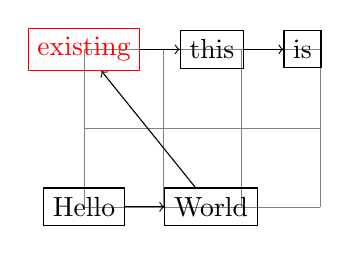
\begin{tikzpicture}[node distance=5mm,
                    every node/.style=draw,every join/.style=->]
  \draw [help lines] (0,0) grid (3,2);

  \node[red] (existing) at (0,2) {existing};

  \begin{scope}[start chain]
    \node [draw,on chain,join] {Hello};
    \node [draw,on chain,join] {World};
    \chainin (existing) [join];
    \node [draw,on chain,join] {this};
    \node [draw,on chain,join] {is};
  \end{scope}
\end{tikzpicture}
\end{codeexample}

    Here is an example where nodes are positioned using a matrix and then
    connected using a chain
    %
{\catcode`\|=12
\begin{codeexample}[]
\begin{tikzpicture}[every node/.style=draw]
  \matrix [matrix of nodes,column sep=5mm,row sep=5mm]
  {
    |(a)|           World & |(b) [circle]|             peace \\
    |(c)|           be    & |(d) [isosceles triangle]| would \\
    |(e) [ellipse]| great & |(f)|                      ! \\
  };

  % (the `scopes' library needs to be loaded to make the following work)
  { [start chain,every on chain/.style={join=by ->}]
    \chainin (a);
    \chainin (b);
    \chainin (d);
    \chainin (c);
    \chainin (e);
    \chainin (f);
  }
\end{tikzpicture}
\end{codeexample}
}
    %
\end{command}


\subsection{Joining Nodes on a Chain}

\begin{key}{/tikz/join=\opt{|with |\meta{with} }\opt{|by |\meta{options}}}
    When this key is given to any node on a chain (except possibly for the
    first node), an |edge| command is added after the node. The |with| part
    specifies which node should be used for the start point of the edge; if the
    |with| part is omitted, the |\tikzchainprevious| is used. This |edge|
    command gets the \meta{options} as parameter and the current node as its
    target. If there is no previous node and no |with| is given, no |edge|
    command gets executed.
    %
    \begin{stylekey}{/tikz/every join}
        This style is executed each time this command is used.
    \end{stylekey}

    Note that it makes sense to call this option several times for a node, in
    order to connect it to several nodes. This is especially useful for joining
    in branches, see the next section.
    %
\begin{codeexample}[]
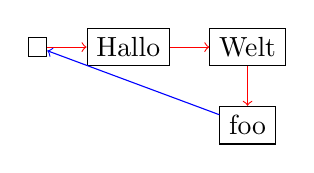
\begin{tikzpicture}[start chain,node distance=5mm,
                    every join/.style={->,red}]
  \node [draw,on chain,join] {};
  \node [draw,on chain,join] {Hallo};
  \node [draw,on chain,join] {Welt};
  \node [draw,on chain=going below,
         join,join=with chain-1 by {blue,<-}] {foo};
\end{tikzpicture}
\end{codeexample}
    %
\end{key}


\subsection{Branches}

A \emph{branch} is a chain that (typically only temporarily) extends an
existing chain. The idea is the following: Suppose we are constructing a chain
and at some node |x| there is a fork. In this case, one (or even more) branches
starts at this fork. For each branch a chain is created, but the first node on
this chain should be~|x|. For this, it is useful to use |\chainin| on the node
|x| to make it part of the different branch chains and to name the branch
chains in some way that reflects the name of the main chain.

The |start branch| option provides a shorthand for doing exactly what was just
described.

\begin{key}{/tikz/start branch=\meta{branch name}\opt{\meta{direction}}}
    This key is used in the same manner as the |start chain| command, however,
    the effect is slightly different:
    %
    \begin{itemize}
        \item This option may only be used if some chain is already active and
            there is a (last) node on this chain. Let us call this node the
            \meta{fork node}.
        \item The chain is not just called \meta{branch name}, but
            \meta{current chain}|/|\meta{branch name}. For instance, if the
            \meta{fork node} is part of the chain called |trunk| and the
            \meta{branch name} is set to |left|, the complete chain name of the
            branch is |trunk/left|. The \meta{branch name} must be given, there
            is no default value.
        \item The \meta{fork node} is automatically ``chained into'' the branch
            chain as its first node. Thus, for the first node on the branch
            that you provide, the |join| option will cause it to be connected
            to the fork node.
    \end{itemize}
    %
\begin{codeexample}[]
\begin{tikzpicture}[every on chain/.style=join,every join/.style=->,
                    node distance=2mm and 1cm]
  { [start chain=trunk]
    \node [on chain] {A};
    \node [on chain] {B};

    { [start branch=numbers going below]
      \node [on chain] {1};
      \node [on chain] {2};
      \node [on chain] {3};
    }
    { [start branch=greek going above]
      \node [on chain] {$\alpha$};
      \node [on chain] {$\beta$};
      \node [on chain] {$\gamma$};
    }

    \node [on chain,join=with trunk/numbers-end,join=with trunk/greek-end] {C};
    { [start branch=symbols going below]
      \node [on chain] {$\star$};
      \node [on chain] {$\circ$};
      \node [on chain] {$\int$};
    }
  }
\end{tikzpicture}
\end{codeexample}
    %
\end{key}

\begin{key}{/tikz/continue branch=\meta{branch name}\opt{\meta{direction}}}
    This option works like the |continue chain| option, only \meta{current
    chain}|/|\meta{branch name} is used as the chain name, rather than just
    \meta{branch name}.
    %
\begin{codeexample}[]
\begin{tikzpicture}[every on chain/.style=join,every join/.style=->,
                    node distance=2mm and 1cm]
  { [start chain=trunk]
    \node [on chain] {A};
    \node [on chain] {B};
    { [start branch=numbers going below] } % just a declaration,
    { [start branch=greek   going above] } % we will come back later
    \node [on chain] {C};

    % Now come the branches...
    { [continue branch=numbers]
      \node [on chain] {1};
      \node [on chain] {2};
    }
    { [continue branch=greek]
      \node [on chain] {$\alpha$};
      \node [on chain] {$\beta$};
    }
  }
\end{tikzpicture}
\end{codeexample}
    %
\end{key}
